% (c) 2012 Dimitrios Vrettos - d.vrettos@gmail.com
% (c) 2017 Daniele Zambelli - daniele.zambelli@gmail.com
% 
% Tutti i grafici per il capitolo relativo alla divisibilità_scomposizione
% di polinomi

\newcommand{\divisionenumerica}{%
\begin{tikzpicture}[x=5mm,y=5mm, ampersand replacement=\&]%, font=\small]
\begin{scope}[font=\ttfamily]
\matrix (a) [matrix of nodes, anchor=south]{
1\&4\&7\&4\\
1\&2\&{}\&3\&6\\
\&2\&7\\
\&2\&4\\
\&{}\&3\\};
\end{scope}

\draw(a-1-4.north west)--(a-2-4.south west);
\draw(a-2-4.north west)--(a-2-5.north east);
\draw(a-2-1.south west)--(a-2-3.south east);
\draw(a-4-2.south west)--(a-4-3.south east);

\begin{scope}[color=blue!50!black]
\node (d) at (-4.5, 5) {dividendo};
\node (r) at (-3, 0.5) {resto};
\node (di) at (4.5, 5) {divisore};
\node (q) at (5, 3) {quoziente};
\end{scope}

\begin{scope}[->]
\draw (d.east)--(a-1-1.west);
\draw (r.east)--(a-5-3.west);
\draw (di.west)--(a-1-4.east);
\draw (q.west)--(a-2-5.east);
\end{scope}
\end{tikzpicture}
}

\newcommand{\divpola}{%
\begin{tikzpicture}[ampersand replacement=\&]%, font=\footnotesize]

\matrix  (a) [matrix of  nodes, anchor=south, text depth=1mm]{
$3x^4$\&$-4x^3$\&$+0x^2$\&$+5x$\&$-1$ \&$3x^2$\&$+0x$\&$-1$\\};

\draw(a-1-6.north west)--(a-1-6.south west);
\draw(a-1-6.south west)--(a-1-8.south east);

\begin{scope}[color=blue!50!black]%font=\scriptsize]
 \node[above] (d) at (a-1-3.north) {dividendo};
 \node[below] (r) at (a-1-3.south) {Spazio per i calcoli};
 \node [above](di) at (a-1-7.north) {divisore};
 \node [below] (q) at (a-1-7.south) {quoziente};
\end{scope}
\end{tikzpicture}
}

\newcommand{\divpolb}{%
\begin{tikzpicture}[ampersand replacement=\&]%, font=\footnotesize]
 \pgfsetmatrixrowsep{5mm}

% \matrix  (a) [matrix of  nodes, anchor=south, minimum width=9mm, ,nodes={text 
% depth=1mm}]{
\matrix (a) [matrix of nodes, anchor=south, minimum width=9mm, text 
depth=1mm]{
$3x^4$\&$-4x^3$\&$+0x^2$\&$+5x$\&$-1$ \&$3x^2$\&$+0x$\&$-1$\\
\&\&\&\&\&$x^2$\\};

 \draw(a-1-6.north west)--(a-2-6.south west);
 \draw(a-1-6.south west)--(a-1-8.south east);

 \begin{scope}[->, red!50!black]
\draw (a-1-1.north) .. controls +(up:8mm) and +(up:10mm).. 
      node[below] {$:$} (a-1-6);
\draw (a-1-6.south) -- (a-2-6.north);
 \end{scope}
\end{tikzpicture}
}

\newcommand{\divpolc}{%
\begin{tikzpicture}[ampersand replacement=\&]
\pgfsetmatrixrowsep{2mm}

\matrix (a) [matrix of nodes, anchor=south, minimum width=9mm, text 
depth=1mm]{
$3x^4$\&$-4x^3$\&$+0x^2$\&$+5x$\&$-1$ \&$3x^2$\&$+0x$\&$-1$\\
$-3x^4$\&$-0x^3$\&$+x^2$\&\&\&$x^2$\\};

 \draw(a-1-6.north west)--(a-2-6.south west);
\draw(a-1-6.south west)--(a-1-8.south east);

\begin{scope}[->,red, dashed]
 \draw (a-1-7.south) -- (a-2-6.east);
  \draw (a-2-6.west) -- (a-2-3.east);
 \end{scope}

\end{tikzpicture}
}

\newcommand{\divpold}{%
\begin{tikzpicture}[ampersand replacement=\&]
\matrix  (a) [matrix of  nodes, anchor=south, minimum width=9mm, text 
depth=1mm]{
$3x^4$\&$-4x^3$\&$+0x^2$\&$+5x$\&$-1$ \&$3x^2$\&$+0x$\&$-1$\\
$-3x^4$\&$-0x^3$\&$+x^2$\&\&{}\&$x^2$\\
{}\&$-4x^3$\&$+x^2$\&$+5x$\&$-1$\\};
\draw(a-1-6.north west)--(a-2-6.south west);
\draw(a-1-6.south west)--(a-1-8.south east);
\draw (a-2-1.south west) -- (a-2-5.south east);
\end{tikzpicture}
}

\newcommand{\divpole}{%
\begin{tikzpicture}[ampersand replacement=\&]
\matrix  (a) [matrix of  nodes, anchor=south, minimum width=9mm, nodes={text 
depth=2.5mm}]{
$3x^4$\&$-4x^3$\&$+0x^2$\&$+5x$\&$-1$ \&$3x^2$\&$+0x$\&$-1$\\
$-3x^4$\&$-0x^3$\&$+x^2$\&\&{}\&$x^2$\&$-\displaystyle\frac{4}{3}x$\\
{}\&$-4x^3$\&$+x^2$\&$+5x$\&$-1$\\};
\draw(a-1-6.north west)--(a-2-6.south west);
  \draw(a-1-6.south west)--(a-1-8.south east);
 \draw (a-2-1.south west) -- (a-2-5.south east);
\end{tikzpicture}
}

\newcommand{\divpolf}{%
\begin{tikzpicture}[ampersand replacement=\&]
\matrix  (a) [matrix of  nodes, anchor=south, minimum width=9mm, ,nodes={text 
depth=2.5mm}]{
$3x^4$\&$-4x^3$\&$+0x^2$\&$+5x$\&$-1$ \&$3x^2$\&$+0x$\&$-1$\\
$-3x^4$\&$-0x^3$\&$+x^2$\&\&{}\&$x^2$\&$-\displaystyle\frac{4}{3}x$\\
{}\&$-4x^3$\&$+x^2$\&$+5x$\&$-1$\\
{}\&$-4x^3$\&$+0x^2$\&$-\displaystyle\frac{4}{3}x$\&{}\\
{}\&\&$x^2$\&$+\displaystyle\frac{11}{3}x$\&$-1$\\};
\draw(a-1-6.north west)--(a-2-6.south west);
\draw(a-1-6.south west)--(a-1-8.south east);
\draw (a-2-1.south west) -- (a-2-5.south east);
\draw (a-4-2.south west) -- (a-4-5.south east);
\end{tikzpicture}
}

\newcommand{\divpolg}{%
\begin{tikzpicture}[ampersand replacement=\&]

\matrix  (a) [matrix of  nodes, anchor=south, minimum width=9mm, ,nodes={text 
depth=2.5mm}]{
$3x^4$\&$-4x^3$\&$+0x^2$\&$+5x$\&$-1$ \&$3x^2$\&$+0x$\&$-1$\\
$-3x^4$\&$-0x^3$\&$+x^2$\&\&{}\&$x^2$\&$-\displaystyle\frac{4}{3}
x$\&$+\displaystyle\frac{1}{3}$\\
{}\&$-4x^3$\&$+x^2$\&$+5x$\&$-1$\\
{}\&$+4x^3$\&$+0x^2$\&$-\displaystyle\frac{4}{3}x$\&{}\\
{}\&\&$x^2$\&$+\displaystyle\frac{11}{3}x$\&$-1$\\
{}\&\&$-x^2$\&$+0x$\&$+\displaystyle\frac{1}{3}$\\
{}\&\&\&$+\displaystyle\frac{11}{3}x$\&$-\displaystyle\frac{2}{3}$\\};
\draw(a-1-6.north west)--(a-2-6.south west);
\draw(a-1-6.south west)--(a-1-8.south east);
\draw (a-2-1.south west) -- (a-2-5.south east);
\draw (a-4-2.south west) -- (a-4-5.south east);
\draw (a-6-4.south west) -- (a-6-5.south east);
\end{tikzpicture}
}

\newcommand{\divdue}{%
\begin{tikzpicture}[ampersand replacement=\&]
\matrix  (a) [matrix of  nodes, anchor=south, minimum width=9mm,nodes={text 
depth=1mm}]{
$x^3$\&$-2x^2$\&$+x$\&$-2$ \&$x^2$\&$+0x$\&$+1$\\
$-x^3$\&$-0x^2$\&$-x$\&{}\&$x$\&$-2$\\
{}\&$-2x^2$\&$+0x$\&$-2$\\
{}\&$-2x^2$\&$+0x$\&$-2$\\
\&\&\&$0$\&{}\\
};
\draw(a-1-5.north west)--(a-2-5.south west);
\draw(a-1-5.south west)--(a-1-7.south east);
\draw (a-2-1.south west) -- (a-2-4.south east);
\draw (a-4-2.south west) -- (a-4-4.south east);
\end{tikzpicture}
}

\newcommand{\ruffinia}{
\begin{tikzpicture}[ampersand replacement=\&]

\matrix  (a) [matrix of  nodes, anchor=south, minimum width=9mm,nodes={text 
depth=0mm}]{
$ 3x^4$ \& $+8x^3$ \& $+9x^2$ \& $ +4x$ \& $ -5$  \& $ x   $ \& $+2$    \&  {}   
\&  {}  
\\
$-3x^4$ \& $-6x^3$ \&    {}   \&   {}   \&   {}   \& $ 3x^3$ \& $+2x^2$ \& $+5x$ 
\& $ 
-6$\\
  {}    \& $+2x^3$ \& $+9x^2$ \&   {}   \&       \\
  {}    \& $-2x^3$ \& $-4x^2$ \&   {}   \&   {}   \&   {}    \&  R$=+7$\\
  {}    \&   {}    \& $+5x^2$ \& $ +4x$ \&   {}  \\
  {}    \&   {}    \& $-5x^2$ \& $-10x$ \&   {}  \\
  {}    \&   {}    \& $ {}  $ \& $ -6x$ \& $ -5$ \\
  {}    \&   {}    \& $ {}  $ \& $ +6x$ \& $+12$ \\
  {}    \&   {}    \& $ {}  $ \& $ {} $ \& $+7$ \\
};

\draw(a-1-5.north east)--(a-9-5.south east);
\draw(a-2-6.north west)--(a-2-9.north east);
\draw (a-2-1.south west) -- (a-2-3.south east);
\draw (a-4-2.south west) -- (a-4-4.south east);
\draw (a-6-3.south west) -- (a-6-5.south east);
\draw (a-8-4.south west) -- (a-8-5.south east);
%  \draw (a-4-2.south west) -- (a-4-4.south east);
\end{tikzpicture}
}

\newcommand{\ruffinib}{
\begin{tikzpicture}[ampersand replacement=\&, %minimum size=6mm,
data/.style={
rectangle,
minimum size=6mm,
top color=white,
bottom color=red!50!black!20,
% font=\small
},
interm/.style={
rectangle,
minimum size=6mm,
draw=black,
% font=\small
},
result/.style={
rectangle, rounded corners=3mm,
minimum size=6mm,
draw=black,
% font=\small
}]

\matrix  (a) [matrix of  nodes, anchor=south, minimum width=9mm,
              nodes={text depth=0mm}]{
\node[result, data]{$+3$}; \& \node[data]{$+8$}; \& \node[data]{$+9$}; \& 
\node[data]{$ +4$}; \& \node[data]{$ -5$};  \& {} \&$ 1   $ \& 
\node[data]{$+2$};    
\&  {}   \&  {}  \\
$-3$ \& \node[interm]{$-6$}; \&  {}  \&  {}   \& {} \&  {}   \& $ 3$ \& $+2$ \& 
$+5$ \& $ 
-6$\\
 {}    \& \node[result]{$+2$}; \& $+9$ \&   {}   \& {} \& \\
 {}    \& $-2$ \& \node[interm]{$-4$}; \&   {}   \& {} \&  {}   \&   {}    \&  
R$=+7$\\
 {}    \&  {}  \& \node[result]{$+5$}; \& $ +4$ \&   {} \& {} \&\\
 {}    \&  {}  \& $-5$ \& \node[interm]{$-10$}; \&   {} \& {} \&\\
 {}    \&  {}  \& ${}$ \& \node[result]{$ -6$}; \& $ -5$ \& {} \&\\
 {}    \&  {}  \& ${}$ \& $ +6$ \& \node[interm]{$+12$}; \& {} \&\\
 {}    \&  {}  \& ${}$ \& $ {}$ \& \node[result]{$+7$}; \& {} \&\\
};

\draw(a-1-6.north east)--(a-9-6.south east);
\draw(a-2-7.north west)--(a-2-10.north east);
\draw (a-2-1.south west) -- (a-2-3.south east);
\draw (a-4-2.south west) -- (a-4-4.south east);
\draw (a-6-3.south west) -- (a-6-5.south east);
\draw (a-8-4.south west) -- (a-8-6.south east);
%  \draw (a-4-2.south west) -- (a-4-4.south east);
\end{tikzpicture}
}

% \newcommand{\ruffinic}{%
% \begin{tikzpicture}[font=\small,x=8mm, y=8mm, minimum size=10mm]
% 
% \node (a0) at (0,0) {};
% \node (a1) at (1,0) {1};
% \node (a2) at (2,0) {$-3$};
% \node (a3) at (3,0) {1};
% 
% \node(a4) at (0,-1) {1};
% \node (a5) at (1,-1) {};
% \node (a6) at (2,-1) {};
% \node (a7) at (3,-1) {};
% 
% \node (a8) at (0,-2) {};
% \node (a9) at (1,-2) {};
% \node (a10) at (2,-2) {};
% \node (a11) at (3,-2) {};
% 
% \draw (a0.north east)--(a8.south east);
%  \draw (a4.south west)--(a7.south east);
% \draw (a2.north east)--(a10.south east);
% 
% \node (b) at (2,3) {Coefficienti numerici del divendo};
% \node[text width=3.4cm] (c) at (-4,0){Termine noto del divisore cambiato di 
% segno};
% \node[text width=3cm] (d) at (7,0) {Termine noto del dividendo};
% 
% \begin{scope}[->, red]
% \foreach \x in {a1.north, a2.north, a3.north}
% 	\draw (b.south)--(\x);
% \draw (c) -- (a4.west);
% \draw (d)-- (a3.east);
% \end{scope}
% 
% \end{tikzpicture}
% }

% \newcommand{\ruffinid}{%
% \begin{tikzpicture}[font=\small,x=8mm, y=8mm, minimum size=10mm]
% 
% \node (a0) at (0,0) {};
% \node (a1) at (1,0) {1};
% \node (a2) at (2,0) {$-3$};
% \node (a3) at (3,0) {1};
% 
% \node(a4) at (0,-1) {1};
% \node (a5) at (1,-1) {};
% \node (a6) at (2,-1) {};
% \node (a7) at (3,-1) {};
% 
% \node (a8) at (0,-2) {};
% \node (a9) at (1,-2) {1};
% \node (a10) at (2,-2) {};
% \node (a11) at (3,-2) {};
% 
% \draw (a0.north east)--(a8.south east);
%  \draw (a4.south west)--(a7.south east);
% \draw (a2.north east)--(a10.south east);
% 
% \draw[->,red] (a1.south)--(a9.north);
% 
% \end{tikzpicture}
% }

\newcommand{\ruffinic}{%
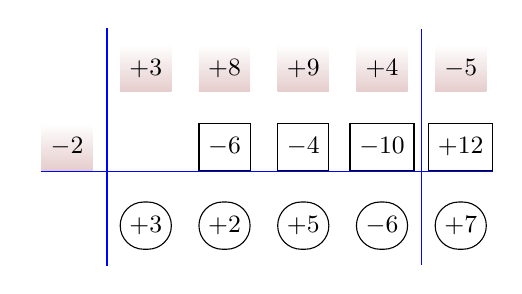
\begin{tikzpicture}[font=\small, %minimum size=6mm,
data/.style={
rectangle,
minimum size=6mm,
top color=white,
bottom color=red!50!black!20,
% font=\small
},
interm/.style={
rectangle,
minimum size=6mm,
draw=black,
% font=\small
},
result/.style={
rectangle, rounded corners=3mm,
minimum size=6mm,
draw=black,
% font=\small
},
x=10mm, y=10mm, minimum size=10mm]

\node (a0) at (0,0) {};
\node [data](a1) at (1,0) {$+3$};
\node [data](a2) at (2,0) {$+8$};
\node [data](a3) at (3,0) {$+9$};
\node [data](a4) at (4,0) {$+4$};
\node [data](a5) at (5,0) {$-5$};

\node [data](a6) at (0,-1) {$-2$};
\node (a7) at (1,-1) {};
\node [interm](a8) at (2,-1) {$-6$};
\node [interm](a9) at (3,-1) {$-4$};
\node [interm](a10) at (4,-1) {$-10$};
\node [interm](a11) at (5,-1) {+12};

\node (a12) at (0,-2) {};
\node [result](a13) at (1,-2) {$+3$};
\node [result](a14) at (2,-2) {$+2$};
\node [result](a15) at (3,-2) {$+5$};
\node [result](a16) at (4,-2) {$-6$};
\node [result](a17) at (5,-2) {$+7$};

\begin{scope}[blue]
\draw (a0.north east)--(a12.south east);
 \draw (a6.south west)--(a11.south east);
% \draw (a4.north east)--(a16.south east);
\draw (4.5, 0.5)--(4.5, -2.5);
\end{scope}

% \matrix (a)[matrix of nodes, nodes in empty cells,
%             nodes={ text width=8mm, text depth=1mm, text centered}]
% {
%  {}  & \node [data]{$+3$}; & \node [data]{$+8$}; & \node [data]{$+9$}; & 
% \node 
% [data]{$+4$};  & \node [data]{$-5$}; \\
% $-2$ &  {}  & $-6$ & $-4$ & $-10$ & $+12$ \\
%  {}  & $+3$ & $+2$ & $+5$ & $-6$  & $+7$  \\
% };  
% \begin{scope}[blue]
% \draw(a-1-2.north west)--(a-3-2.south west);
% \draw(a-2-1.south west)--(a-2-6.south east);
% \draw(a-1-5.north east)--(a-3-5.south east);
% \end{scope}
\end{tikzpicture}
}

\newcommand{\ruffinid}{%
% \usepgflibrary{arrows.meta}

\begin{tikzpicture}[font=\small, x=10mm, y=10mm, minimum size=10mm]

% \begin{tikzpicture}[font=\small,x=8mm, y=8mm, minimum size=10mm]

\node (a0) at (0,0) {};
\node (a1) at (1,0) {$+3$};
\node (a2) at (2,0) {$+8$};
\node (a3) at (3,0) {$+9$};
\node (a4) at (4,0) {$+4$};
\node (a5) at (5,0) {$-5$};

\node (a6) at (0,-1) {$-2$};
\node (a7) at (1,-1) {};
\node (a8) at (2,-1) {$-6$};
\node (a9) at (3,-1) {$-4$};
\node (a10) at (4,-1) {$-10$};
\node (a11) at (5,-1) {+12};

\node (a12) at (0,-2) {};
\node (a13) at (1,-2) {$+3$};
\node (a14) at (2,-2) {$+2$};
\node (a15) at (3,-2) {$+5$};
\node (a16) at (4,-2) {$-6$};
\node (a17) at (5,-2) {$+7$};

\begin{scope}[blue]
\draw (a0.north east)--(a12.south east);
 \draw (a6.south west)--(a11.south east);
% \draw (a4.north east)--(a16.south east);
\draw (4.5, 0.5)--(4.5, -2.5);
\end{scope}

% \draw (a0.north east)--(a12.south east);
% \draw (a6.south west)--(a11.south east);
% \draw (a4.north east)--(a16.south east);

\draw [-{Stealth[length=3mm, open, round]}, 
       green, loosely dashed, line width=2pt](1.3, 0) -- (1.3, -2);
% \draw [-{Stealth[length=3mm, open, round]}, 
%       red, solid, line width=2pt] 
%       (a6.east) [xshift=-0.5cm] -- (a13.north) [yshift=-0.5cm] -- (a8.west) 
[xshift=+0.5cm];
\draw [-{Stealth[length=3mm, open, round]}, 
       red!50, dotted, line width=2pt] 
       (0.3, -1.2) -- (1, -1.8) -- (1.7, -1.2);
\draw [-{Stealth[length=3mm, open, round]}, 
       green, loosely dashed, line width=2pt](2.3, 0) -- (2.3, -2);
\draw [-{Stealth[length=3mm, open, round]}, 
       red!50, dotted, line width=2pt] 
       (0.3, -1.2) -- (2, -1.8) -- (2.7, -1.2);
\draw [-{Stealth[length=3mm, open, round]}, 
       green, loosely dashed, line width=2pt](3.3, 0) -- (3.3, -2);
\draw [-{Stealth[length=3mm, open, round]}, 
       red!50, dotted, line width=2pt] 
       (0.3, -1.2) -- (3, -1.8) -- (3.7, -1.2);
\draw [-{Stealth[length=3mm, open, round]}, 
       green, loosely dashed, line width=2pt](4.3, 0) -- (4.3, -2);
\draw [-{Stealth[length=3mm, open, round]}, 
       red!50, dotted, line width=2pt] 
       (0.3, -1.2) -- (4, -1.8) -- (4.7, -1.2);
\draw [-{Stealth[length=3mm, open, round]}, 
       green, loosely dashed, line width=2pt](5.3, 0) -- (5.3, -2);

\end{tikzpicture}
}

\newcommand{\ruffinie}{%
\begin{tikzpicture}[font=\small, %minimum size=6mm,
data/.style={
rectangle,
minimum size=6mm,
top color=white,
bottom color=red!50!black!20,
% font=\small
},
interm/.style={
rectangle,
minimum size=6mm,
draw=black,
% font=\small
},
result/.style={
rectangle, rounded corners=3mm,
minimum size=6mm,
draw=black,
% font=\small
},
x=10mm, y=10mm, minimum size=10mm]


% \begin{tikzpicture}[font=\small,x=8mm, y=8mm, minimum size=10mm]

\node (a0) at (0,0) {};
\node [data](a1) at (1,0) {};
\node [data](a2) at (2,0) {};
\node [data](a3) at (3,0) {};
\node [data](a4) at (4,0) {};
\node [data](a5) at (5,0) {};

\node [data](a6) at (0,-1) {};
\node (a7) at (1,-1) {};
\node [interm](a8) at (2,-1) {};
\node [interm](a9) at (3,-1) {};
\node [interm](a10) at (4,-1) {};
\node [interm](a11) at (5,-1) {};

\node (a12) at (0,-2) {};
\node [result](a13) at (1,-2) {};
\node [result](a14) at (2,-2) {};
\node [result](a15) at (3,-2) {};
\node [result](a16) at (4,-2) {};
\node [result](a17) at (5,-2) {};

% \draw (a0.north east)--(a12.south east);
%  \draw (a6.south west)--(a11.south east);
% \draw (a4.north east)--(a16.south east);

\begin{scope}[blue]
\draw (a0.north east)--(a12.south east);
 \draw (a6.south west)--(a11.south east);
% \draw (a4.north east)--(a16.south east);
\draw (4.5, 0.5)--(4.5, -2.5);
\end{scope}

\draw [-{Stealth[length=3mm, open, round]}, 
       green, loosely dashed, line width=2pt](1.4, 0) -- (1.4, -2);
\draw [-{Stealth[length=3mm, open, round]}, 
       red!50, dotted, line width=2pt] 
       (0.3, -1.2) -- (1, -1.8) -- (1.7, -1.2);
\draw [-{Stealth[length=3mm, open, round]}, 
       green, loosely dashed, line width=2pt](2.4, 0) -- (2.4, -2);
\draw [-{Stealth[length=3mm, open, round]}, 
       red!50, dotted, line width=2pt] 
       (0.3, -1.2) -- (2, -1.8) -- (2.7, -1.2);
\draw [-{Stealth[length=3mm, open, round]}, 
       green, loosely dashed, line width=2pt](3.4, 0) -- (3.4, -2);
\draw [-{Stealth[length=3mm, open, round]}, 
       red!50, dotted, line width=2pt] 
       (0.3, -1.2) -- (3, -1.8) -- (3.7, -1.2);
\draw [-{Stealth[length=3mm, open, round]}, 
       green, loosely dashed, line width=2pt](4.4, 0) -- (4.4, -2);
\draw [-{Stealth[length=3mm, open, round]}, 
       red!50, dotted, line width=2pt] 
       (0.3, -1.2) -- (4, -1.8) -- (4.7, -1.2);
\draw [-{Stealth[length=3mm, open, round]}, 
       green, loosely dashed, line width=2pt](5.4, 0) -- (5.4, -2);

\end{tikzpicture}
}

\newcommand{\scompfattnum}{%
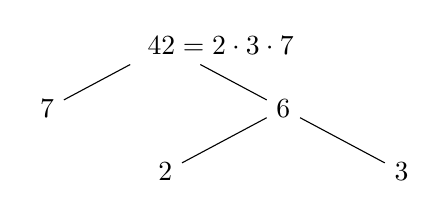
\begin{tikzpicture}[level/.style={sibling distance=30mm, level distance=8mm}]
\node {$\qquad \qquad 42 = 2 \cdot 3 \cdot 7$}
  child {node {$7$}}
  child {node {$6$}
    child {node {$2$}}
    child {node {$3$}}
  };
\end{tikzpicture}
}

\newcommand{\scompfattpol}{%
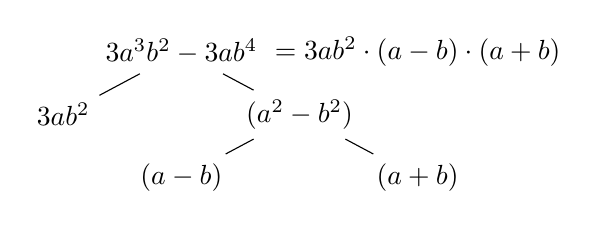
\begin{tikzpicture}[level/.style={sibling distance=30mm, level distance=8mm}]
\node {$3a^{3}b^{2}-3ab^{4}$}
  child {node {$3ab^2$}}
  child {node {$(a^2 -b^2)$}
    child {node {$(a-b)$}}
    child {node {$(a+b)$}}
  };

\draw (3, 0) node {$= 3ab^2 \cdot (a-b) \cdot (a+b)$};
\end{tikzpicture}
}
% 
% \newcommand{\ruffini}[4]{%
%   % 
%   \def \rigaa{#1}
%   \def \rigab{#2}
%   \def \rigac{#3}
%   \def \dim{#4}
% %   \begin{tikzpicture}[x=5mm, y=5mm]
% 
%     \foreach \val [count = \ival] in \rigaa 
%       \node at (\ival*2, 0) {\(\val\)};
%     \foreach \val [count = \ival] in \rigab 
%       \node at (\ival*2, -1) {\(\val\)};
%     \foreach \val [count = \ival] in \rigac 
%     \node at (\ival*2, -2) {\(\val\)};
% 
%     \begin{scope}[blue!50!black]
%       \draw (3, .5) -- (3, -2.5);
%       \draw (\dim*2 - 1, .5) -- (\dim*2 - 1, -2.5);
%       \draw (1, -1.5) -- (\dim*2+1, -1.5);
%     \end{scope}
% %   \end{tikzpicture}
% }

\newcommand{\scompruffiniaa}{%
  \disegno{
    \ruffini{~, +1, +1, -10, +8}
            {+1, {}, +1, ~~+2, -8}
            {{}, +1, +2, ~~-8, ~~~0}
            {5}
  }
}

\newcommand{\scompruffiniab}{%
  \disegno{
    \ruffini{~, +1, +2, -8}
            {+2, ~, +2, +8}
            {~, +1, +4, ~~~0}
            {4}
  }
}

\newcommand{\scompruffiniac}{
  \disegno{
    \ruffini{~, +1, +1, -10, +8}
            {+1, {}, +1, ~~+2, -8}
            {{}, +1, +2, ~~-8, ~~~0}
            {5}
    \begin{scope}[yshift=-10mm]
    \ruffini{}
            {+2, ~, +2, ~~+8}
            {~, +1, +4, ~~~~~0}
            {4}
    \end{scope}
  }
}

\newcommand{\scompruffiniad}{
  \disegno{
    \ruffini{~, +1, -5, -7, +29, +30}
            {-1, {}, -1, +6, +~~1, -30}
            {{}, +1, -6, ~~-1, +30, ~~~~~0}
            {6}
    \begin{scope}[yshift=-10mm]
      \ruffini{}
              {-2, ~, -2, +16, -30}
              {~, +1, -8, +15, ~~~~~0}
              {5}
      \begin{scope}[yshift=-10mm]
        \ruffini{}
                {+3, ~, +3, +15}
                {~, +1, -5, ~~~~~0}
                {4}
      \end{scope}
    \end{scope}
  }
}

\newcommand{\scompruffinib}{%
\begin{tikzpicture}[x=5mm, y=5mm, ampersand replacement=\&]
\matrix (a)[matrix of nodes, nodes in empty cells,nodes={ text width=8mm, text 
depth=1mm, text centered}]{
\&1\&$-5$\&$-7$\&29\&30\\
$-1$\&\&$-1$\&6\&1\&$-30$\\
\&1\&$-6$\&$-1$\&30\&0\\
};  
\begin{scope}[blue]
\draw(a-1-2.north west)--(a-3-1.south east);
\draw(a-2-1.south west)--(a-2-6.south east);
\draw(a-1-5.north east)--(a-3-5.south east);
      \end{scope}
\end{tikzpicture}
}

\newcommand{\scompruffinic}{%
\begin{tikzpicture}[x=5mm, y=5mm, ampersand replacement=\&]
\matrix (a)[matrix of nodes, nodes in empty cells,nodes={ text width=8mm, text 
depth=1mm, text centered}]{
\&1\&$-6$\&$-1$\&30\\
$-2$\&\&$-2$\&16\&$-30$\\
\&1\&$-8$\&$15$\&0\\
};  
\begin{scope}[blue]
\draw(a-1-2.north west)--(a-3-1.south east);
\draw(a-2-1.south west)--(a-2-5.south east);
\draw(a-1-4.north east)--(a-3-4.south east);
      \end{scope}
\end{tikzpicture}
}

\newcommand{\scompruffinid}{%
  \disegno{
    \ruffini{~, +6, -1, -2}
            {-\frac{1}{2}, ~, -3, +2}
            {~, +6, -4, ~~~0}
            {4}
  }
}
% 
% \newcommand{\scompruffinid}{%
% \begin{tikzpicture}[x=5mm, y=5mm, ampersand replacement=\&]
% \matrix (a)[matrix of nodes, nodes in empty cells,nodes={ text width=8mm, text 
% depth=1mm, text centered}]{
% \&6\&$-1$\&$-2$\\
% $-\frac{1}{2}$\&\&$-3$\&2\\
% \&6\&$-4$\&0\\
% };  
% \begin{scope}[blue]
% \draw(a-1-2.north west)--(a-3-1.south east);
% \draw(a-2-1.south west)--(a-2-4.south east);
% \draw(a-1-3.north east)--(a-3-3.south east);
%       \end{scope}
% \end{tikzpicture}
% }

\newcommand{\binomogeneiruffinia}{%
\begin{tikzpicture}[x=5mm, y=5mm, ampersand replacement=\&]
\matrix (a)[matrix of nodes, nodes in empty cells,
            nodes={ text width=8mm, text depth=1mm, text centered}]
{
     \& $1$ \& $ 0$ \& $0$    \& $+a^3$ \\
$-a$ \&     \& $-a$ \& $+a^2$ \& $-a^3$ \\
     \& $1$ \& $-a$ \& $+a^2$ \& $0$ \\
};  
\begin{scope}[blue]
\draw(a-1-2.north west)--(a-3-2.south west);
\draw(a-2-1.south west)--(a-2-5.south east);
\draw(a-1-4.north east)--(a-3-4.south east);
\end{scope}
\end{tikzpicture}
}

\newcommand{\binomogeneiruffinib}{%
\begin{tikzpicture}[x=5mm, y=5mm, ampersand replacement=\&]
\matrix (a)[matrix of nodes, nodes in empty cells,
            nodes={ text width=8mm, text depth=1mm, text centered}]
{
     \& $1$ \& $ 0$ \& $0$    \& $-a^3$ \\
$+a$ \&     \& $+a$ \& $+a^2$ \& $+a^3$ \\
     \& $1$ \& $+a$ \& $+a^2$ \& $0$ \\
};  
\begin{scope}[blue]
\draw(a-1-2.north west)--(a-3-2.south west);
\draw(a-2-1.south west)--(a-2-5.south east);
\draw(a-1-4.north east)--(a-3-4.south east);
\end{scope}
\end{tikzpicture}
}

\newcommand{\scompruffinie}{%
  \disegno{
    \ruffini{~, +1, ~~0, -7, -6}
            {-1, {}, -1, +1, +6}
            {{}, +1, -1, -6, ~~~0}
            {5}
  }
}
% 
% \newcommand{\scompruffinie}{%
% \begin{tikzpicture}[x=5mm, y=5mm, ampersand replacement=\&]
% \matrix (a)[matrix of nodes, nodes in empty cells,
%             nodes={ text width=8mm, text depth=1mm, text centered}]{
% \&1\&0\&$-7$\&$-6$\\
% $-1$\&\&$-1$\&1\&6\\
% \&1\&$-1$\&$-6$\&0\\
% };  
% \begin{scope}[blue]
% \draw(a-1-2.north west)--(a-3-1.south east);
% \draw(a-2-1.south west)--(a-2-5.south east);
% \draw(a-1-4.north east)--(a-3-4.south east);
%       \end{scope}
% \end{tikzpicture}
% }

\newcommand{\esedivisionea}{%
\begin{tikzpicture}[ampersand replacement=\&]
\matrix (a) [matrix of nodes, anchor=south, minimum width=9mm, ,nodes={text 
depth=2.5mm}]{
$7x^4$\&$+0x^3$\&$-5x^2$\&$+x$\&$-1$ \&$2x^2$\&$+0x$\&$-1$\\
{}\&{}\&$\ldots$\&{}\&{}\&$\displaystyle\frac{7}{2}x$\&\ldots\\
{}\&{}\&$-\displaystyle\frac{3}{2}x^2$\&$+x$\&$-1$\\
{}\&{}\&{}\&\ldots\&{}\\
\&\&\&$x$\&$-\displaystyle\frac{7}{4}$\\
};
\draw(a-1-6.north west)--(a-2-6.south west);
\draw(a-1-6.south west)--(a-1-8.south east);
 \draw (a-2-1.south west) -- (a-2-5.south east);
 \draw (a-4-2.south west) -- (a-4-5.south east);
\end{tikzpicture}
}

\newcommand{\esedivisioneb}{%
\begin{tikzpicture}[ampersand replacement=\&]
\matrix (a) [matrix of nodes, anchor=south, minimum width=9mm, ,nodes={text 
depth=2.5mm}]{
$3a^3$\&$+3a^2b$\&$+4ab^2$\&$-2b^3$\&$a$\&$-3b$\\
{}\&{}\&$\ldots$\&{}\&$3a^2$\&-\ldots\\
};
\draw(a-1-5.north west)--(a-2-5.south west);
\draw(a-1-5.south west)--(a-1-6.south east);
\end{tikzpicture}
}

\newcommand{\diffcubia}{%
\begin{tikzpicture}[x=5mm, y=5mm, ampersand replacement=\&]
\matrix (a)[matrix of nodes, nodes in empty cells,nodes={ text width=8mm, text 
depth=1mm, text centered}]{
\&1\&0\&0\&$-8$\\
2\&\&2\&4\&8\\
\&1\&2\&4\&/\\
};  
\begin{scope}[blue]
\draw(a-1-2.north west)--(a-3-1.south east);
\draw(a-2-1.south west)--(a-2-5.south east);
\draw(a-1-4.north east)--(a-3-4.south east);
      \end{scope}
\end{tikzpicture}
}

\newcommand{\diffcubib}{%
\begin{tikzpicture}[x=5mm, y=5mm, ampersand replacement=\&]
\matrix (a)[matrix of nodes, nodes in empty cells,nodes={ text width=8mm, text 
depth=1mm, text centered}]{
\&1\&0\&0\&27\\
$-3$\&\&$-3$\&9\&$-27$\\
\&1\&$-3$\&9\&/\\
};  
\begin{scope}[blue]
\draw(a-1-2.north west)--(a-3-1.south east);
\draw(a-2-1.south west)--(a-2-5.south east);
\draw(a-1-4.north east)--(a-3-4.south east);
      \end{scope}
\end{tikzpicture}
}
